% !TEX program = XeLaTeX
% !TEX encoding = UTF-8
\documentclass[10pt]{beamer}
\usetheme{metropolis}

% Support Chinese Characters
\usepackage[scheme=plain,nofonts,noindent,UTF8]{ctexcap}
\renewcommand\CJKfamilydefault{\CJKsfdefault}
\setCJKmainfont[BoldFont=FandolSong-Bold.otf,ItalicFont=FandolKai-Regular.otf]{FandolSong-Regular.otf}
\setCJKsansfont[BoldFont=FandolHei-Bold.otf]{FandolHei-Regular.otf}
\setCJKmonofont{FandolFang-Regular.otf}

\usepackage{pgfplots}
\usetikzlibrary{shapes}

% left-aligned description lists
\defbeamertemplate{description item}{align left}{\insertdescriptionitem\hfill}

% yay, matching colors!
\definecolor{alert}{HTML}{EB811B}
\definecolor{example}{HTML}{14B03D}

% DIY QED Symbol
\newcommand*{\QED}{\hfill\ensuremath{\blacksquare}}%

\title{Estimating the Upper Bound of the Cover Size of the Complete Subtree Method}
\subtitle{Big Data Security}
\date{\today}
\author{李卓倩, 王帅朝, Raziur Rahman Totha, Julien Schmidt}
\institute{Shanghai Jiao Tong University}

\begin{document}

\maketitle

\begin{frame}{The Problem}
  \begin{itemize}
    \item Broadcast Encryption
    \item Stateless Receivers
    \item Revocation Scheme
  \end{itemize}
  %\pause

  \begin{block}{Goal}
  Sender sending message to a group of users, in which a subset is considered revoked and should not be able to obtain the content.
  \end{block}
  \pause

  \begin{exampleblock}{Example}
    Pay-TV
  \end{exampleblock}
\end{frame}

% Dalit and Moni Naor and Jeff Lotspiech
\begin{frame}{The Subset-Cover Revocation Framework}
D. Naor, M. Naor, and J. Lotspiech. ``Revocation and
Tracing Schemes for Stateless Receivers''. \textit{Annual International Cryptology Conference}. Springer Berlin Heidelberg, 2001.
%\pause

  \begin{itemize}
    \item Provide condition for the security of revocation schemes
    \item Separation between long-lived keys and short-lived keys
    \item Separation of tracing mechanism from revocation algorithm
    \item \alert{Subset-Cover Algorithms}
    \pause
    \begin{enumerate}
      \item Receivers partitioned into multiple subsets
      \item Cover all non-revoked receivers with disjoint subsets
    \end{enumerate}
    \vspace{-0.5em}
    \begin{itemize}
      \item No assumed upper bound of revoked receivers
    \end{itemize}
  \end{itemize}
  %\pause

  \resizebox{\textwidth}{!}{
    \begin{tabular}{|c|c|c|c|c|}
    \hline
    Method & \alert{Cover Size} & Keys per Receiver & Processing Time & Decryptions \\
    \hline
    \alert{Complete Subtree} & \alert{$r \log{\frac{n}{r}}$} & $\log{n}$ & $O(\log\log{n})$ & 1 \\
    Subset Difference & $2r - 1$ & $\frac{1}{2}\log^2{n}$ & $O(\log{n})$ & 1 \\
    \hline
    \end{tabular}
  }
\end{frame}

\begin{frame}[t]{The Complete Subtree Method}
  \only<1>{
    $S_j$ = Set of (sub-) child leaves
  }\only<2>{
    {\color{example} $S_1 = \{u_1, u_2, u_3, u_4, u_5, u_6, u_7, u_8\}$}
  }\only<3>{
    {\color{example} $S_2 = \{u_1, u_2, u_3, u_4\}$}
  }\only<4>{
    {\color{example} $S_5 = \{u_3, u_4\}$}
  }\only<5>{
    {\color{example} $S_{11} = \{u_4\}$}
  }\\
  \vspace{1.7em}
  \begin{center}
    \only<1>{
    \begin{tikzpicture}[overlay,level distance=1.4cm,
  level 1/.style={sibling distance=5.6cm},
  level 2/.style={sibling distance=2.8cm},
  level 3/.style={sibling distance=1.4cm}]
      \tikzstyle{m}=[circle, draw, minimum size=4mm,inner sep=0pt]
      \node [m] {\tiny1}
        child {node [m] {\tiny2}
          child {node [m] {\tiny4}
            child {node [rectangle,draw] {$u_1$}}
            child {node [rectangle,draw] {$u_2$}}
          }
          child {node [m] {\tiny5}
            child {node [rectangle,draw] {$u_3$}}
            child {node [rectangle,draw] {$u_4$}}
          }
        }
        child {node [m] {\tiny3}
          child {node [m] {\tiny6}
            child {node [rectangle,draw] {$u_5$}}
            child {node [rectangle,draw] {$u_6$}}
          }
          child {node [m] {\tiny7}
            child {node [rectangle,draw] {$u_7$}}
            child {node [rectangle,draw] {$u_8$}}
          }
        };
    \end{tikzpicture}
    }\only<2>{
    \begin{tikzpicture}[overlay,level distance=1.4cm,
  level 1/.style={sibling distance=5.6cm},
  level 2/.style={sibling distance=2.8cm},
  level 3/.style={sibling distance=1.4cm}]
      \tikzstyle{m}=[circle, draw, minimum size=4mm,inner sep=0pt]
      \node [m,fill=example,text=white] (a) {\tiny1}
        child {node [m] {\tiny2}
          child {node [m] {\tiny4}
            child {node [rectangle,draw,fill=lightgray] (b) {$u_1$}}
            child {node [rectangle,draw,fill=lightgray] {$u_2$}}
          }
          child {node [m] {\tiny5}
            child {node [rectangle,draw,fill=lightgray] {$u_3$}}
            child {node [rectangle,draw,fill=lightgray] {$u_4$}}
          }
        }
        child {node [m] {\tiny3}
          child {node [m] {\tiny6}
            child {node [rectangle,draw,fill=lightgray] {$u_5$}}
            child {node [rectangle,draw,fill=lightgray] {$u_6$}}
          }
          child {node [m] {\tiny7}
            child {node [rectangle,draw,fill=lightgray] {$u_7$}}
            child {node [rectangle,draw,fill=lightgray] (c) {$u_8$}}
          }
        };

      \coordinate (A) at ([yshift=.2cm]a.north);
      \coordinate (B) at ([xshift=-.2cm]b.south west);
      \coordinate (C) at ([xshift=.2cm]c.south east);

      \draw[dashed,example,thick] plot[smooth cycle] coordinates {(A) (B) (C)};
    \end{tikzpicture}
    }\only<3>{
    \begin{tikzpicture}[overlay,level distance=1.4cm,
  level 1/.style={sibling distance=5.6cm},
  level 2/.style={sibling distance=2.8cm},
  level 3/.style={sibling distance=1.4cm}]
      \tikzstyle{m}=[circle, draw, minimum size=4mm,inner sep=0pt]
      \node [m] {\tiny1}
        child {node [m,fill=example,text=white] (a) {\tiny2}
          child {node [m] {\tiny4}
            child {node [rectangle,draw,fill=lightgray] (b) {$u_1$}}
            child {node [rectangle,draw,fill=lightgray] {$u_2$}}
          }
          child {node [m] {\tiny5}
            child {node [rectangle,draw,fill=lightgray] {$u_3$}}
            child {node [rectangle,draw,fill=lightgray] (c) {$u_4$}}
          }
        }
        child {node [m] {\tiny3}
          child {node [m] {\tiny6}
            child {node [rectangle,draw] {$u_5$}}
            child {node [rectangle,draw] {$u_6$}}
          }
          child {node [m] {\tiny7}
            child {node [rectangle,draw] {$u_7$}}
            child {node [rectangle,draw] {$u_8$}}
          }
        };

      \coordinate (A) at ([yshift=.2cm]a.north);
      \coordinate (B) at ([xshift=-.2cm]b.south west);
      \coordinate (C) at ([xshift=.2cm]c.south east);

      \draw[dashed,example,thick] plot[smooth cycle] coordinates {(A) (B) (C)};
    \end{tikzpicture}
    }\only<4>{
    \begin{tikzpicture}[overlay,level distance=1.4cm,
  level 1/.style={sibling distance=5.6cm},
  level 2/.style={sibling distance=2.8cm},
  level 3/.style={sibling distance=1.4cm}]
      \tikzstyle{m}=[circle, draw, minimum size=4mm,inner sep=0pt]
      \node [m] {\tiny1}
        child {node [m] {\tiny2}
          child {node [m] {\tiny4}
            child {node [rectangle,draw] {$u_1$}}
            child {node [rectangle,draw] {$u_2$}}
          }
          child {node [m,fill=example,text=white] (a) {\tiny5}
            child {node [rectangle,draw,fill=lightgray] (b) {$u_3$}}
            child {node [rectangle,draw,fill=lightgray] (c) {$u_4$}}
          }
        }
        child {node [m] {\tiny3}
          child {node [m] {\tiny6}
            child {node [rectangle,draw] {$u_5$}}
            child {node [rectangle,draw] {$u_6$}}
          }
          child {node [m] {\tiny7}
            child {node [rectangle,draw] {$u_7$}}
            child {node [rectangle,draw] {$u_8$}}
          }
        };

      \coordinate (A) at ([yshift=.2cm]a.north);
      \coordinate (B) at ([xshift=-.2cm]b.south west);
      \coordinate (C) at ([xshift=.2cm]c.south east);

      \draw[dashed,example,thick] plot[smooth cycle] coordinates {(A) (B) (C)};
    \end{tikzpicture}
    }\only<5>{
    \begin{tikzpicture}[overlay,level distance=1.4cm,
  level 1/.style={sibling distance=5.6cm},
  level 2/.style={sibling distance=2.8cm},
  level 3/.style={sibling distance=1.4cm}]
      \tikzstyle{m}=[circle, draw, minimum size=4mm,inner sep=0pt]
      \node [m] {\tiny1}
        child {node [m] {\tiny2}
          child {node [m] {\tiny4}
            child {node [rectangle,draw] {$u_1$}}
            child {node [rectangle,draw] {$u_2$}}
          }
          child {node [m]  {\tiny5}
            child {node [rectangle,draw] {$u_3$}}
            child {node [rectangle,draw,fill=example] (a) {$u_4$}}
          }
        }
        child {node [m] {\tiny3}
          child {node [m] {\tiny6}
            child {node [rectangle,draw] {$u_5$}}
            child {node [rectangle,draw] {$u_6$}}
          }
          child {node [m] {\tiny7}
            child {node [rectangle,draw] {$u_7$}}
            child {node [rectangle,draw] {$u_8$}}
          }
        };

      \draw (a) [dashed,example,thick] circle [radius=.4cm];
    \end{tikzpicture}
    }
  \end{center}
\end{frame}

\begin{frame}[t]{The Complete Subtree Method}
  $\color{red} \mathcal{R} = \{u_2, u_5, u_6\}$\\
  \only<1>{
    \textit{Steiner Tree $ST(\mathcal{R})$}
  }
  \only<2>{
    $\color{example} \mathcal{N}\setminus\mathcal{R} = S_8 \cup S_5 \cup S_7 $
  }
  \begin{center}
    \only<1>{
    \begin{tikzpicture}[overlay,level distance=1.4cm,
  level 1/.style={sibling distance=5.6cm},
  level 2/.style={sibling distance=2.8cm},
  level 3/.style={sibling distance=1.4cm}]
      \tikzstyle{m}=[circle, draw, minimum size=4mm,inner sep=0pt]
      \tikzstyle{r}=[color=red,text=black,thin,edge from parent/.style={red,thick,draw}]
      \tikzstyle{n}=[black,thin,edge from parent/.style={black,thin,draw}]

      \node [m,color=red,text=black] {\tiny1}
        child[r] {node [m] {\tiny2}
          child[r] {node [m] {\tiny4}
            child[n] {node [rectangle,draw] {$u_1$}}
            child[r] {node [rectangle,draw,fill=red] {$u_2$}}
          }
          child[n] {node [m]  {\tiny5}
            child {node [rectangle,draw] {$u_3$}}
            child {node [rectangle,draw] {$u_4$}}
          }
        }
        child[r] {node [m] {\tiny3}
          child[r] {node [m] {\tiny6}
            child[r] {node [rectangle,draw,fill=red] {$u_5$}}
            child[r] {node [rectangle,draw,fill=red] {$u_6$}}
          }
          child[n] {node [m] {\tiny7}
            child {node [rectangle,draw] {$u_7$}}
            child {node [rectangle,draw] {$u_8$}}
          }
        };
    \end{tikzpicture}
    }\only<2>{
    \begin{tikzpicture}[overlay,level distance=1.4cm,
  level 1/.style={sibling distance=5.6cm},
  level 2/.style={sibling distance=2.8cm},
  level 3/.style={sibling distance=1.4cm}]
      \tikzstyle{m}=[circle, draw, minimum size=4mm,inner sep=0pt]
      \tikzstyle{r}=[color=red,text=black,thin,edge from parent/.style={red,thick,draw}]
      \tikzstyle{n}=[black,thin,edge from parent/.style={black,thin,draw}]

      \node [m,color=red,text=black] {\tiny1}
        child[r] {node [m] {\tiny2}
          child[r] {node [m] {\tiny4}
            child[n] {node [rectangle,draw,fill=example] (a) {$u_1$}}
            child[r] {node [rectangle,draw,fill=red] {$u_2$}}
          }
          child[n] {node [m,fill=example,text=white] (b) {\tiny5}
            child {node [rectangle,draw,fill=lightgray] (c) {$u_3$}}
            child {node [rectangle,draw,fill=lightgray] (d) {$u_4$}}
          }
        }
        child[r] {node [m] {\tiny3}
          child[r] {node [m] {\tiny6}
            child[r] {node [rectangle,draw,fill=red] {$u_5$}}
            child[r] {node [rectangle,draw,fill=red] {$u_6$}}
          }
          child[n] {node [m,fill=example,text=white] (e) {\tiny7}
            child {node [rectangle,draw,fill=lightgray] (f) {$u_7$}}
            child {node [rectangle,draw,fill=lightgray] (g) {$u_8$}}
          }
        };

      \draw (a) [dashed,example,thick] circle [radius=.4cm];

      \coordinate (B) at ([yshift=.2cm]b.north);
      \coordinate (C) at ([xshift=-.2cm]c.south west);
      \coordinate (D) at ([xshift=.2cm]d.south east);
      \draw[dashed,example,thick] plot[smooth cycle] coordinates {(B) (C) (D)};

      \coordinate (E) at ([yshift=.2cm]e.north);
      \coordinate (F) at ([xshift=-.2cm]f.south west);
      \coordinate (G) at ([xshift=.2cm]g.south east);
      \draw[dashed,example,thick] plot[smooth cycle] coordinates {(E) (F) (G)};
    \end{tikzpicture}
    }
  \end{center}
\end{frame}

\begin{frame}{The Cover Size Upper Bound}
  \textit{The cover size is at most}
  \begin{center}
    \scalebox{2}{
      $\mathbf{r \cdot \log{\frac{n}{r}}}$
    }
  \end{center}
  \pause

  $\Rightarrow$ How many \textbf{subset keys} have to be transmitted in the \textbf{worst case}?
  \pause

  \vspace{1em}

  \setbeamertemplate{description item}[align left]
  \begin{description}[$S_1, ..., S_w$, $S_j \subseteq \mathcal{N}$ .]
    \item[$\mathcal{N}$] Set of receivers (devices)
    \item[$S_1, ..., S_w$, $S_j \subseteq \mathcal{N}$] Subsets
    \item[$\mathcal{R}$] Set of revoked receivers
    \item[$\mathcal{N}\setminus\mathcal{R} = \bigcup_{j=1}^{m} S_{i_j}$] Set of non-revoked receivers is a partition of subsets
    \item[$n = \left\vert{\mathcal{N}}\right\vert$]
    \item[$r = \left\vert{\mathcal{R}}\right\vert$]
  \end{description}

\end{frame}

\begin{frame}{Proof Idea}
\begin{block}{Observation}
\alert{The number of required subsets is equal to the number of nodes with degree $1$ in $ST(\mathcal{R})$}
\end{block}
\vskip 1cm

\begin{block}{Upper Bound $C_{max}(n,r)$:}
The max. cover size for $n$ receivers in total of which $r$ are revoked
\begin{itemize}
  \item Trivially $C_{max}(n,0) = 1$
  \item $0 < r \leq n \Longrightarrow$ Induction
\end{itemize}
\end{block}

\end{frame}

\begin{frame}{Induction Base}
  \metroset{block=fill}
  \begin{block}{Depth $k=1$:}
  \vskip 0.3cm
  $n = 2^k = 2$\\

    \begin{center}
      \begin{minipage}{.4\textwidth}
        $\mathbf{r=1}$:\\
        \begin{center}
        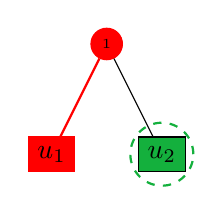
\begin{tikzpicture}[level distance=1.4cm,
        level 1/.style={sibling distance=1.4cm}]
            \tikzstyle{m}=[circle,draw,fill=white,minimum size=4mm,inner sep=0pt]
            \tikzstyle{r}=[color=red,text=black,thin,edge from parent/.style={red,thick,draw}]
            \tikzstyle{n}=[black,thin,edge from parent/.style={black,thin,draw}]

            \node [m,color=red,text=black] {\tiny1}
              child[r] {node [rectangle,draw,fill=red] {$u_1$}}
              child[n] {node [rectangle,draw,fill=example] (a) {$u_2$}};

            \draw (a) [dashed,example,thick] circle [radius=.4cm];
        \end{tikzpicture}\\
        \alert{$C_{max}(2,1) = 1 = 1 \cdot \log\frac{2}{1}$}
        \end{center}
      \end{minipage}
      \begin{minipage}{.4\textwidth}
        $\mathbf{r=2}$:\\
        \begin{center}
        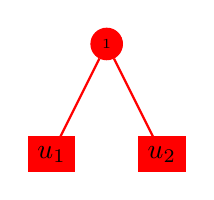
\begin{tikzpicture}[level distance=1.4cm,
        level 1/.style={sibling distance=1.4cm}]
            \tikzstyle{m}=[circle,draw,fill=white,minimum size=4mm,inner sep=0pt]
            \tikzstyle{r}=[color=red,text=black,thin,edge from parent/.style={red,thick,draw}]
            \tikzstyle{n}=[black,thin,edge from parent/.style={black,thin,draw}]

            \node [m,color=red,text=black] {\tiny1}
              child[r] {node [rectangle,draw,fill=red] {$u_1$}}
              child[r] {node [rectangle,draw,fill=red] {$u_2$}};
        \end{tikzpicture}\vspace{0.3cm}\\
        \alert{$C_{max}(2,2) = 0 = 2 \cdot \log\frac{2}{2}$}
        \end{center}
      \end{minipage}
    \end{center}
  \end{block}
\end{frame}

\begin{frame}{Induction Hypothesis}
  To prove: $r \cdot \log{\frac{n}{r}}$
  \begin{itemize}
    \item $k = \log(n)$
    \item $\log(\frac{n}{r}) = \log({n})-\log({r}) = k - \log(r)$
  \end{itemize}

  \vskip 1cm
  \begin{minipage}{.25\textwidth}
    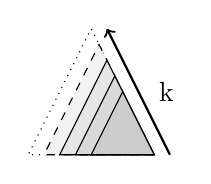
\begin{tikzpicture}
      \draw[dotted] (0,0) -- (-.8,1.6) -- (-1.6,0) -- cycle;
      \filldraw[dashed,draw=black, fill=gray!10] (0,0) -- (-.7,1.4) -- (-1.4,0) -- cycle;
      \filldraw[draw=black, fill=gray!20] (0,0) -- (-.6,1.2) -- (-1.2,0) -- cycle;
      \filldraw[draw=black, fill=gray!30] (0,0) -- (-.5,1) -- (-1,0) -- cycle;
      \filldraw[draw=black, fill=gray!40] (0,0) -- (-.4,.8) -- (-.8,0) -- cycle;

      \draw[->,thick] (0.2,0) -- (-.6,1.6) node [midway, label=right:k] {};
    \end{tikzpicture}
  \end{minipage}
  \begin{minipage}{.5\textwidth}
    \Large
    $C_{max}(2^k,r) \leq r \cdot (k - log(r))$
  \end{minipage}
\end{frame}

\begin{frame}{Induction Step}
  $k \rightarrow k+1$:

  \metroset{block=fill}
  \begin{block}{Case 1: All in one side}
    \begin{center}
      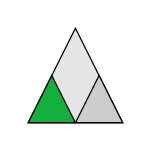
\begin{tikzpicture}
        \filldraw[draw=black, fill=gray!20] (0,0) -- (-.6,1.2) -- (-1.2,0) -- cycle;
        \filldraw[draw=black, fill=example] (-.6,0) -- (-.9,.6) -- (-1.2,0) -- cycle;
        \filldraw[draw=black, fill=gray!40] (0,0) -- (-.3,.6) -- (-.6,0) -- cycle;
      \end{tikzpicture}
    \end{center}
    If all leaves are in a subtree of depth $k$, then the total number of nodes of degree 1 is at most:

    \begin{equation}
      C_{max}(2^{k+1},r) = r \cdot (k - \log r) {\color{example} + 1} \leq r \cdot (k+1 - \log r)
    \end{equation}
  \end{block}
\end{frame}

\begin{frame}{Induction Step}
  \metroset{block=fill}
  \begin{block}{Case 2: $\mathcal{R} = \mathcal{R}_1 \cup \mathcal{R}_2$}
    \begin{center}
      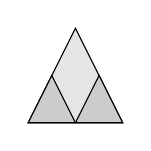
\begin{tikzpicture}
        \filldraw[draw=black, fill=gray!20] (0,0) -- (-.6,1.2) -- (-1.2,0) -- cycle;
        \filldraw[draw=black, fill=gray!40] (-.6,0) -- (-.9,.6) -- (-1.2,0) -- cycle;
        \filldraw[draw=black, fill=gray!40] (0,0) -- (-.3,.6) -- (-.6,0) -- cycle;
      \end{tikzpicture}
    \end{center}

    $\mathcal{R}$ is split among the left ($\mathcal{R}_1$) and right subtree ($\mathcal{R}_2$) of the root. Thus:
    \begin{equation}
      r = r_1 + r_2
    \end{equation}

    By induction at most: $C_{max}(2^{k+1},r) = $
    \begin{equation}\begin{split}
      r_1 \cdot (k - \log r_1) + r_2 \cdot (k - \log r_2) & = r \cdot k - (r_1 \log r_1 + r_2 \log r_2)\\
      & \leq r \cdot (k + 1 - \log r)
    \end{split}\end{equation}
    since $(r_1 \log r_1 + r_2 \log r_2) \geq r \cdot (\log r - 1)$

    \QED
  \end{block}
\end{frame}


\begin{frame}[standout]
  Questions?
\end{frame}

\end{document}
